% backup of examples
% commit 422547a 10/07/2021 by Philippe
% https://github.com/cedric-cnam/WSVPA/commit/422547aa703906e8234eddc51968cfd618400c4f


% introduction.tex

\begin{example}[Running example]\label{ex:running}
We
illustrate our framework with music transcription: given
a \emph{timeline} of musical events with timestamps from an infinite
domain as input, parse it
into a structured music score. Input events
are pairs $\< \mu, \tau>$, with $\mu \in \Sigma$, where $\Sigma$ stands for the
set of MIDI message symbols~\cite{?}
and  $\tau \in \mathbb{Q}$ is a timestamp. Such inputs typically correspond
to the recording of a live performance. The output of parsing
is a sequence of events (or \emph{notes}) $\< \nu, \tau'>$   in
Common Western Music Notation (CWMN)~\cite{Gould11Notation}
where event symbols $\nu$ belong to the domain $\Delta$
of \emph{pitches} (e.g., A4, G5, etc.), and timestamp $\tau'$
belongs to a rhythmic ``grid'' obtained from recursive divisions:
whole notes ($\musWhole$) splitted in halves ($\musHalf$), halves
in quarters ($\musQuarter$), eights ($\musEighth$), etc.
The following concrete sequences
will be used:
\begin{enumerate}
  \item A performance  $I = [ \<\mu_1, 0.07>, \<\mu_2, 0.72>, \<\mu_3, 0.91>, \<\mu_4, 1.05>, \<\mu_5, 1.36>, \<\mu_6, 1.71>]$,
     over interval $[0,2[$,
  \item A score $O =$ 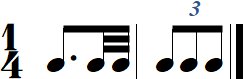
\includegraphics[scale=0.20]{pictures/score5.png}, corresponding to
      a hierarchical structures (measures, tuplets) that can be linearized as a sequence of events
      $[\<\nu_1,0>, \<\nu_2,\frac{3}{4}>, \<\nu_3,\frac{7}{8}>, \<\nu_4,1>, \<\nu_5,\frac{4}{3}>, \<\nu_6\frac{5}{3}>]$
\end{enumerate}
\smallskip

We will show that $O$ is a soution for the
parsing of $I$. Note that several other parsings (e.g.,
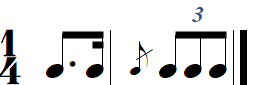
\includegraphics[scale=0.20]{pictures/score4.png}) are possible.
SW-parsing associates a weight value
to each solution, and our framework
aims at selecting the best one with respect to this weight.
\endex
\end{example}


% labels.tex

\begin{example}\label{distance-time}
We return to the music transcription problem (Exemple~\ref{ex:running}). In order to align the
input with a music score, we must take into consideration
the expressive timing of human performance that
results in small time shifts between an input event and the corresponding
notation event.  These shifts can be weighted as the time distance between both,
computed in the tropical semiring as follows.
$$\delta\bigl(\<\mu, \tau>, \<\nu, \tau'>\bigr) =
\left\{
\begin{array}{ll}
   | \tau_1 - \tau_2 | & \mathrm{if}\  \mu \rm{\ corresponds\  to\ } \nu \\
   \zero  & \mathrm{otherwise}
\end{array}
\right.$$
The performance is
$I = [ \<\mu_1, 0.07>, \<\mu_2, 0.72>, \<\mu_3, 0.91>, \<\mu_4, 1.05>, \<\mu_5, 1.36>, \<\mu_6, 1.71>]$,
and the (linearized) score is
$[\<\nu_1,0>, \<\nu_2,\frac{3}{4}>, \<\nu_3,\frac{7}{8}>, \<\nu_4,1>, \<\nu_5,\frac{4}{3}>, \<\nu_6\frac{5}{3}>]$
Assuming the pairwise correspondence of MIDI symbols
$\mu_i$ and notation symbols $\nu_i$, for $i \in [1, 6]$,
the distance between $I$ and $O$ is the  aggregation with $\otimes$
of the pairwise differences between the
timestamps. In the tropical semiring, this yields
$|0.07 - 0| + |0.72 - \frac{3}{4}| + |0.91- \frac{7}{8} | +
|1.05-1| + |1.36-\frac{4}{3}| + |1.71-\frac{5}{3}|= 0.255$.
\endex
\end{example}



% main.tex


\begin{example}\label{ex:SWT}
We build a small weighted transducer model
with two states $q_0$ and $q_1$ that
calculates the distance between the performance $I$ and
the score $O$ of Example~\ref{ex:running}.

If one performed event $\mu_i$  corresponds
to one notated event $\nu_j$ (for instance MIDI code 61 and pitch A4),
the weight value computed by the \SWT is the time distance between both,
(see Example~\ref{distance-time}), and is modeled by
transitions $\wei_{11}$ below.
%
If we meet the music notation symbol '-' that
represents continuation (this occurs for instance in \emph{ties}
$\musQuarter\!\!\!\mathrel{\raisebox{-1.5mm}{$\smile$}}\!\!\!\musEighth$,
or \emph{dots} \musQuarterDotted{}), it is  skipped with no cost (transitions $\wei_{01}$ or weight $\one$).
%transitions
\[
\begin{array}{rclcrcl}
\wei_{11}(q_0, \<\mu, \tau>, \<\nu, \tau'>, q_0) & = & |\tau' - \tau| & \quad &
\wei_{11}(q_1, \<\mu, \tau>, \<\nu, \tau'>, q_0) & = & |\tau' - \tau|\\
\wei_{01}(q_0, \varepsilon, \< \mathsf{-}, \tau'>, q_0) & = & \one & &
\wei_{01}(q_1, \varepsilon, \< \mathsf{-}, \tau'>, q_0) & = & \one\\
\wei_{10}(q_0, \<\mu, \tau>, \varepsilon, q_1) & = & \alpha & & %\multicolumn{3}{l}{\mathrm{for~all~} b \in \Delta}
\end{array}
\]
%
We also want to take performing errors into account, while still being able to compare with the score,
since a performer could, for example, play an unwritten extra note.
\lydia{reformulated this sentence}
%
This is modelled by the transition $\wei_{10}$ with an arbitrary weight value $\alpha \in \Semiring$,
switching from state $q_0$ (normal) to $q_1$ (error).
\philippe{Comprends pas cette phrase}
The transitions in the second column below switch back to the normal state $q_0$.
% the metric computed by the \SWT is the smallest sum of point wise distances
% between dates of input and output events.
At last, we let $q_0$ be the only initial and final state, with
$\init(q_0) = \final(q_0) = \one$, and
$\init(q_1) = \final(q_1) = \zero$.
This \SWT is capable of evaluating the differences between a score and a performance,
all the while ensuring that performance errors are plausible.
%$\init(q_0, d, b) = \final(q_0, d, b) = \one$, and
%$\init(q_1, d, b) = \final(q_1, d, b) = \zero$,
%for all $d \in \Sigma$ and $b \in \Delta$.
\endex
\end{example}



\begin{example}\label{ex:nested-word}
Consider once more the scores of Example~\ref{ex:running}.
$\Deltai$ represents the set of music events of the form $<\nu, \tau>$
where $\nu$ is either a note (e.g. A4), the continuation symbol $-$, or a
rest symbol R. $\Deltac$ and  $\Deltar$ are used to encode the score structure:
Let $\Deltac = \{\langle, \prec\}$ and  $\Deltar = \{\rangle, \succ\}$ where $\langle$
(resp. $\rangle$)
and $\prec$ (resp. $\succ$) correspond to start/end of measures, and start/end of
tuplets. Then  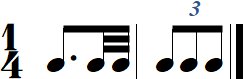
\includegraphics[scale=0.20]{pictures/score5.png}
is encoded with the nested word $\langle \prec 0, \frac{3}{4}, \frac{7}{8} \succ \rangle \langle \prec 1, \frac{4}{3}, \frac{5}{3}  \succ \rangle$
\endex
\end{example}





\begin{example}[Symbolic Weighted Parsing and the transcription problem]
Applied to the music transcription problem, the above formalism
is interpreted as follows:
\begin{enumerate}
\item The \SWT $T$ evaluates a ``fitness measure''  that expresses
 a correspondance between a performance and its notation. See Example~\ref{ex:SWT}.
\item The \SWVPA $A$ expresses a cost related to the music notation. One possibility
 is to relate this cost to the structural complexity: given a set of equivalent
 representations, we aim at choosing the simpler one. For instance
 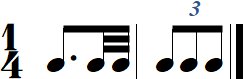
\includegraphics[scale=0.20]{pictures/score5.png} should be favored
 on 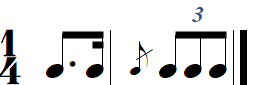
\includegraphics[scale=0.20]{pictures/score4.png}. Costs  can be expressed
 in the grammar as weights associated to each production rule.
 For instance, the following production rules define two possible divisions
 of a time interval into respectively a duplet and a triplet. Each comes with
 a specific cost.
 \[
 \rho_1: q_0 \xrightarrow{0.06} \< q_{1}, q_{2}>,\
 \rho_2: q_0 \xrightarrow{0.12} \< q_{1}, q_{2}, q_{2}>.
 \]
 Further binary divisions of time sub-intervals %represented respectively by~$q_2$ and~$q_3$
 are possible with:
 \[
 \rho_3:\,q_2 \xrightarrow{0.1} \< q_{3}, q_{3}>, \
 \rho_4:\,q_3 \xrightarrow{0.11} \< q_{4}, q_{4}>. \
 \]

Score 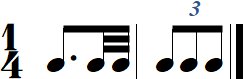
\includegraphics[scale=0.20]{pictures/score5.png} is obtained as follows:
the first measure
 results from the successive applications of  rules $\rho_1$ (division in two)
 and rules $\rho_3$ (division of the second half) in two. The second measure
 is a division in three obtained by rule $\rho_3$. One obtains a parse tree
 that can be linearized in the nested word of Example~\ref{ex:nested-word}.
 \end{enumerate}
Therefore, the framework, applied to the transcription problem, allows to find an optimal
solution that considers both the fitness of the result, and its structural complexity.
\end{example}






\begin{example}[Symbolic Weighted Parsing and the transcription problem]
Applied to the music transcription problem, the above formalism
is interpreted as follows:
\begin{enumerate}

  \item The \SWT $T$ evaluates a ``fitness measure''  that expresses
    a correspondance between a performance and its notation. See Example~\ref{ex:SWT}.
\item The \SWVPA $A$ expresses a cost related to the music notation. One possibility
 is to relate this cost to the structural complexity: given a set of equivalent
 representations, we aim at choosing the simpler one. For instance
 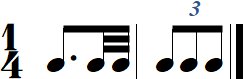
\includegraphics[scale=0.20]{pictures/score5.png} should be favored
 on 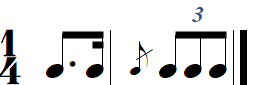
\includegraphics[scale=0.20]{pictures/score4.png}. Costs  can be expressed
 in the grammar as weights associated to each production rule.
 For instance, the following production rules define two possible divisions
 of a time interval into respectively a duplet and a triplet. Each comes with
 a specific cost.
 \[
 \rho_1: q_0 \xrightarrow{0.06} \< q_{1}, q_{2}>,\
 \rho_2: q_0 \xrightarrow{0.12} \< q_{1}, q_{2}, q_{2}>.
 \]
 Further binary divisions of time sub-intervals %represented respectively by~$q_2$ and~$q_3$
 are possible with:
 \[
 \rho_3:\,q_2 \xrightarrow{0.1} \< q_{3}, q_{3}>, \
 \rho_4:\,q_3 \xrightarrow{0.11} \< q_{4}, q_{4}>. \
 \]

Score 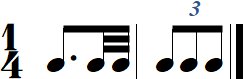
\includegraphics[scale=0.20]{pictures/score5.png} is obtained as follows:
the first measure
 results from the successive applications of  rules $\rho_1$ (division in two)
 and rules $\rho_3$ (division of the second half) in two. The second measure
 is a division in three obtained by rule $\rho_3$. One obtains a parse tree
 that can be linearized in the nested word of Example~\ref{ex:nested-word}.
 \end{enumerate}
Therefore, the framework, applied to the transcription problem, allows to find an optimal
solution that considers both the fitness of the result, and its structural complexity.
\end{example}

